\documentclass[a4paper,10pt]{beamer}

\usepackage{media9}

\usepackage{hyperref}
\usepackage[export]{adjustbox}

\usetheme{Darmstadt}
\useinnertheme{default}
\useoutertheme[footline=empty,subsection=false]{miniframes}
\setbeamertemplate{frametitle}[default][center]
\setbeamertemplate{itemize items}[square]

\setbeamertemplate{blocks}[default]

%\setbeamertemplate{footline}[frame number]
\setbeamertemplate{footline}[text line]{%
}

\setbeamertemplate{background}{%
	\put(5,-270){%
		\parbox{1.16\linewidth}{\tiny Final Project: Brightspace Database Management \hfill \raggedleft\insertframenumber~/ \inserttotalframenumber}
	}
	
}

\setbeamercovered{transparent}

\setbeamertemplate{navigation symbols}{}

\setbeamercolor{block title alerted}{use=structure,fg=white,bg=orange!75!black}
\setbeamercolor{block body alerted}{use=structure,fg=black,bg=orange!10!white}

\setbeamercovered{invisible}

\setbeamertemplate{frametitle}
{
	\nointerlineskip
	\begin{beamercolorbox}[sep=0.3cm,ht=1.8em,wd=\paperwidth]{frametitle}
		\vbox{}\vskip-2ex%
		\strut\vspace*{-0.85cm}\insertframetitle\strut
		\hfill
		\raisebox{-1cm}{
\includegraphics[scale=0.45,trim={0cm 0cm 0 0cm},clip]{logo2_NYU.png}}
		\vskip-0.8ex%
	\end{beamercolorbox}
}

%%%%%%%%%%%% note option %%%%%%%%%%%%
%\setbeameroption{show notes}
%\setbeameroption{show notes on second screen=right}
%%%%%%%%%%%%%%%%%%%%%%%%%%%%%%%%%%%%%

\usepackage{graphicx}
\usepackage{amsmath,amssymb}
\usepackage[latin1]{inputenc}
\usepackage{psfrag}
\usepackage{pgf}
\usepackage{minted}
\usepackage{xcolor}
\usepackage{tcolorbox}
\usepackage{textcomp}
\usepackage{upquote}
\usepackage{media9}


\AtBeginDocument{%
	\def\PYZsq{\textquotesingle}%
}


\usepackage{tikz}
\usetikzlibrary{shapes.geometric, arrows, positioning, shapes.multipart}

\tikzstyle{startstop} = [rectangle, rounded corners, minimum width=2cm, minimum height=1cm,text width=2cm,text centered, draw=black, fill=red!30]
\tikzstyle{process} = [rectangle, minimum width=2cm, minimum height=1cm, text centered, text width=2cm, draw=black, fill=orange!30]
\tikzstyle{decision} = [diamond,aspect=3, minimum width=2cm, minimum height=1cm, text width=2cm,inner sep=0pt,text centered, draw=black, fill=green!30]
\tikzstyle{decision_text} = [rectangle, minimum width=2cm, minimum height=1cm, text width=2cm,inner sep=0pt,text centered]
\tikzstyle{box} = [rectangle, minimum width=0.5cm, minimum height=0.5cm, text width=0.5cm,inner sep=0pt,text centered,draw=black, fill=gray!30]
\tikzstyle{io} = [trapezium, trapezium left angle=70, trapezium right angle=110, trapezium stretches=true,minimum width=2cm, minimum height=1cm, text centered, text width=2cm, draw=black, fill=blue!30]
\tikzstyle{func} = [rectangle split, rectangle split horizontal,rectangle split parts=3,minimum height=1cm, text centered, draw=black, fill=yellow!30,rectangle split empty part width=-6pt]


\tikzstyle{arrow} = [thick,->,>=stealth]

\newcommand\myrule[1]{\multicolumn{1}{c|}{#1}}

\definecolor{light-blue}{RGB}{173,216,230}
\definecolor{yellow}{RGB}{255,255,0}
\definecolor{light-gray}{gray}{0.8}

\newtcbox{\mybox}{nobeforeafter,colback=light-gray,boxrule=0pt,arc=4pt,
	boxsep=0pt,left=6pt,right=6pt,top=6pt,bottom=6pt,width=\width}
\tcbset{ boxrule=0pt,fontupper=\normalsize,colback=light-gray,width=\linewidth,after={\par\noindent}}


\tikzstyle{mybox} = [draw=black, fill=yellow, thick,
rectangle,  inner sep=10pt, inner ysep=20pt]
\tikzstyle{fancytitle} =[fill=black, text=white]


\title{Final Project:\\ Brightspace Database Management}

\author{James Chen \& Shanglin Yang}


\institute{
\includegraphics[scale=1]{logo_NYU.png}}

\date{Instructor: Dr. Anantha Padmanabha}

%\logo{
\includegraphics[scale=0.04]{logo2_NYU.jpg}}


\begin{document}


%%%%%%%%%%%%%%%%%%%%%%%%%%%%%%%%%%%%%%%%%%%%%%%%%%%%%%%%%%%%%%%%%%%%%%%%%%%%%%%%%%%%%%%%%%%%%%%%%%%%%%%%%%%%%
%%%%%%%%%%%%%%%%%%%%%%%%%%%%%%%%%%%%%%%%%%%%%%%%%%%%%%%%%%%%%%%%%%%%%%%%%%%%%%%%%%%%%%%%%%%%%%%%%%%%%%%%%%%%%
\frame[plain]{
	\titlepage
}

\section{Introduction}
\begin{frame}{Overview}
\begin{block}{NYU Brightspace}
\begin{figure}[H]
    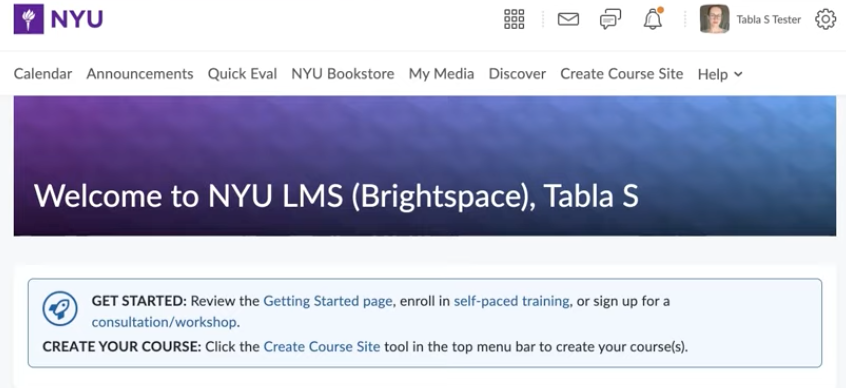
\includegraphics[width=\textwidth]{Intro1.png}
\end{figure}
\end{block}
\end{frame}

\begin{frame}{Sections}
\begin{block}{Table of Content}
\begin{itemize}
    \item \textbf{Introduction}
    \item Diagram
    \item Data generation
    \item Query
\end{itemize}
\end{block}
\end{frame}

\begin{frame}{General Introduction}
\begin{block}{Tech Stack}
\begin{itemize}
    \item MySQL + Excel + Python
    \item Random Dataset
\end{itemize}
\end{block}
\end{frame}


\begin{frame}{General Introduction}
\begin{block}{Why we choose SQL?}
\begin{enumerate}
    \item Data is highly structured and does not change often
    \item Need to perform complex queries
    \item Accuracy rather than performance
    
\end{enumerate}
\end{block}
\end{frame}

\begin{frame}{General Introduction}
\begin{block}{Functions}
\begin{itemize}
    \item Users (Student, Instructor, Admin...)
    \item Courses
    \item Assignment/Quiz/Gradebook
    \item Content
    \item Discussion
    \item Zoom
    \item ...
\end{itemize}
\end{block}
\end{frame}

\begin{frame}{Data Intro}
\begin{block}{Data Intro I}
\begin{figure}[H]
    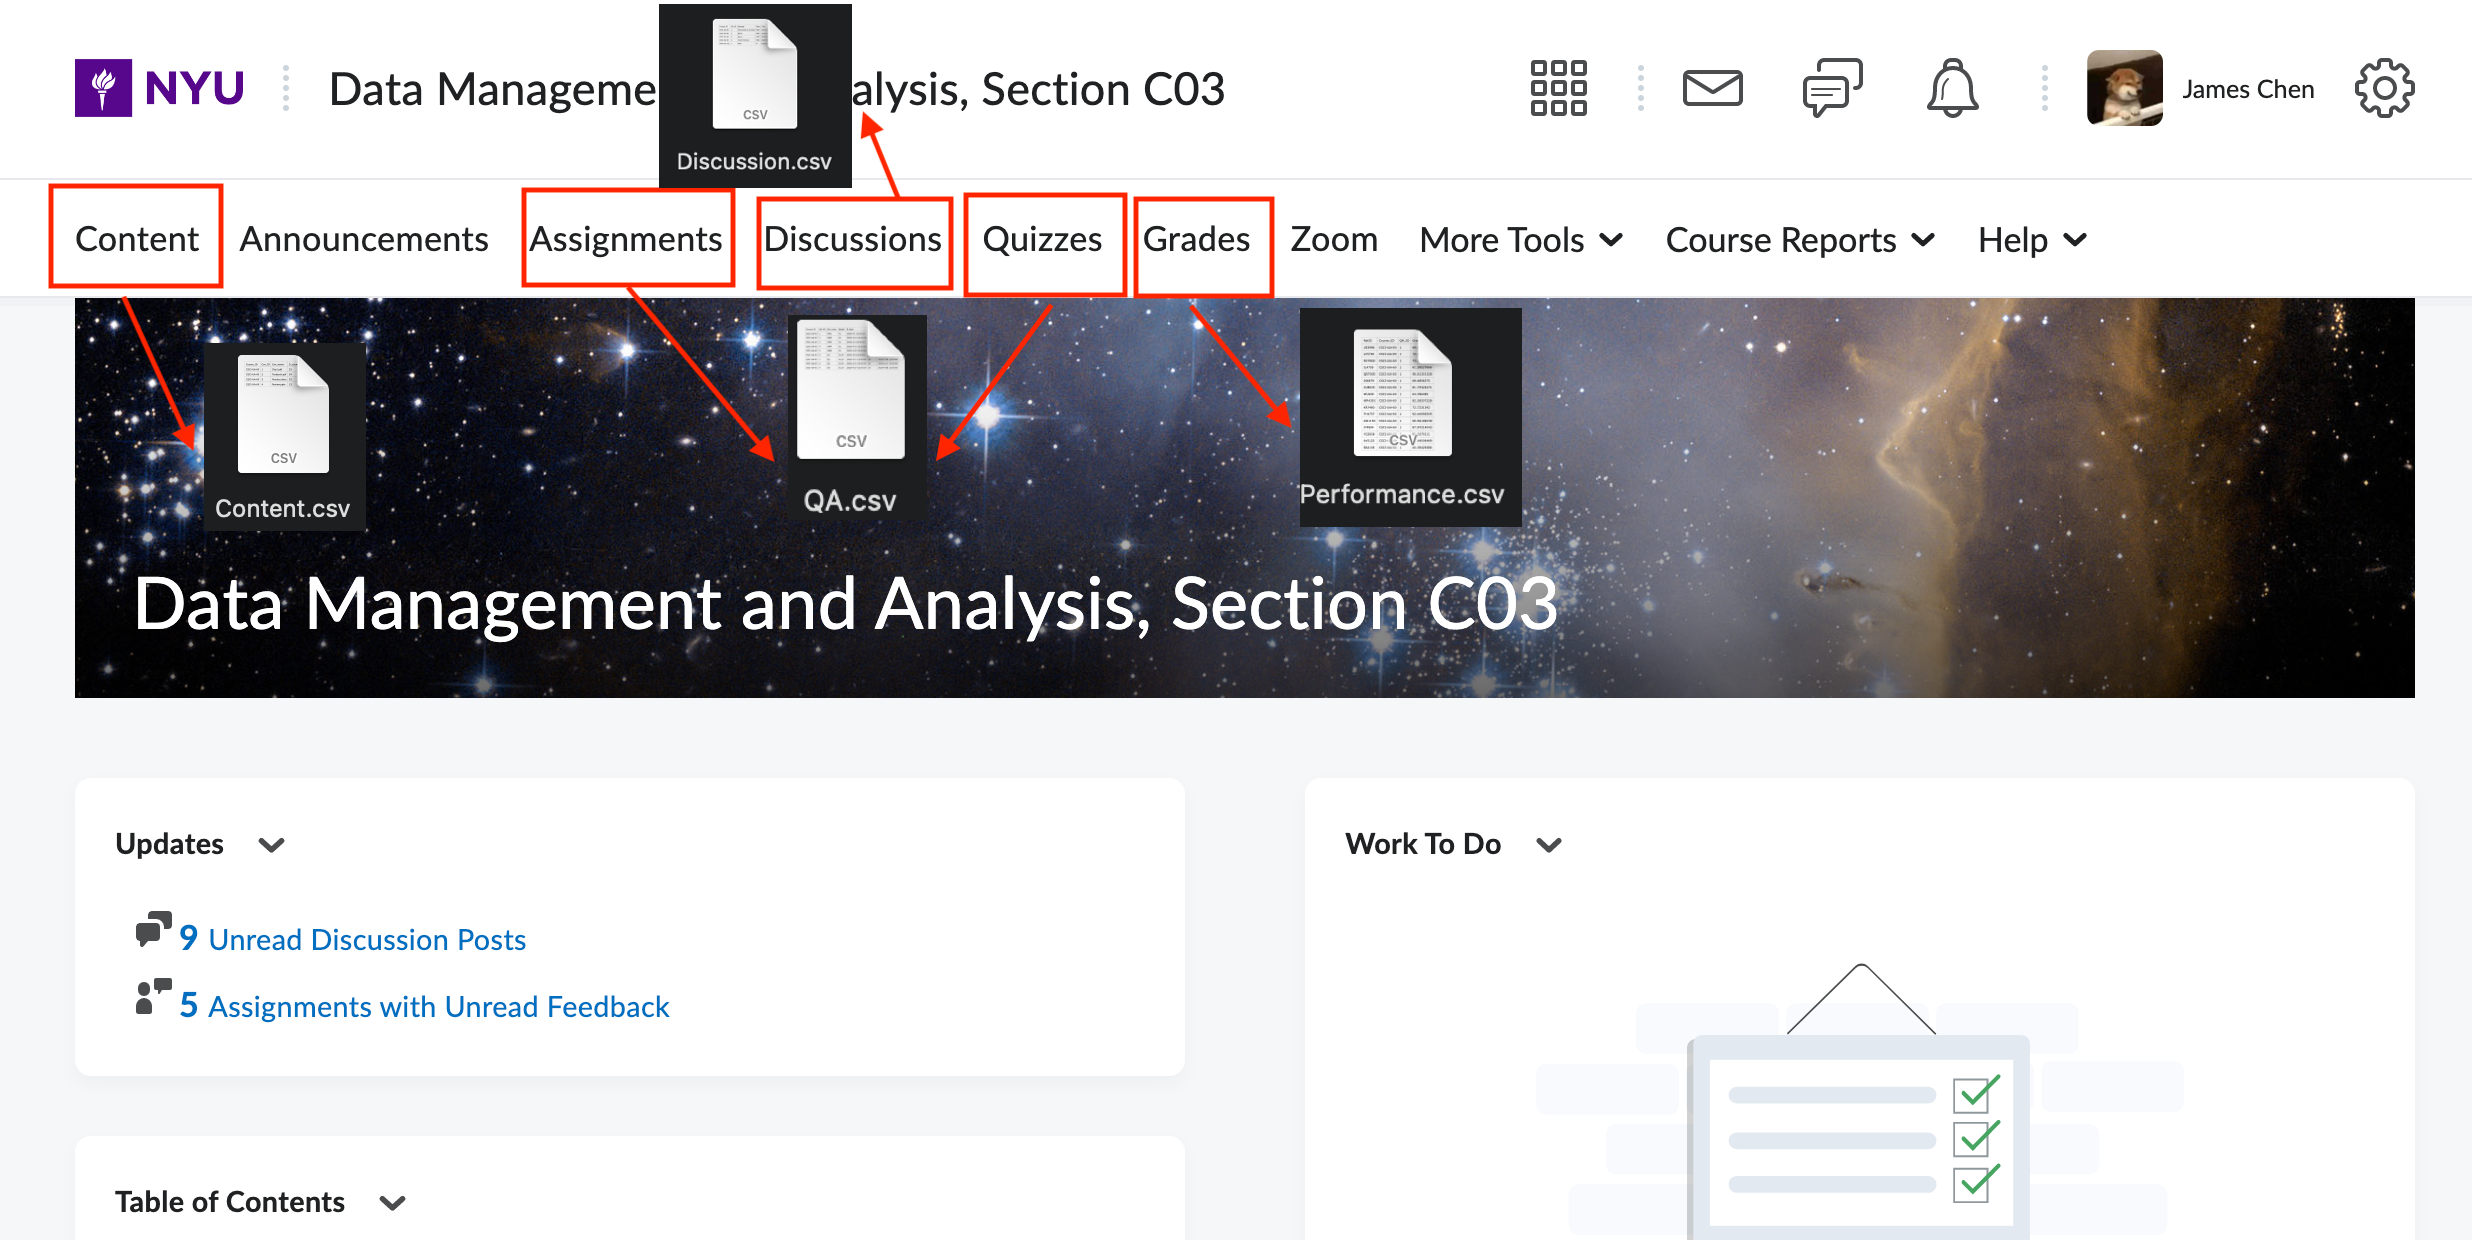
\includegraphics[width=\textwidth]{Intro2.png}
\end{figure}
\end{block}
\end{frame}

\begin{frame}{Data Intro}
\begin{block}{Data Intro II}
\begin{figure}[H]
    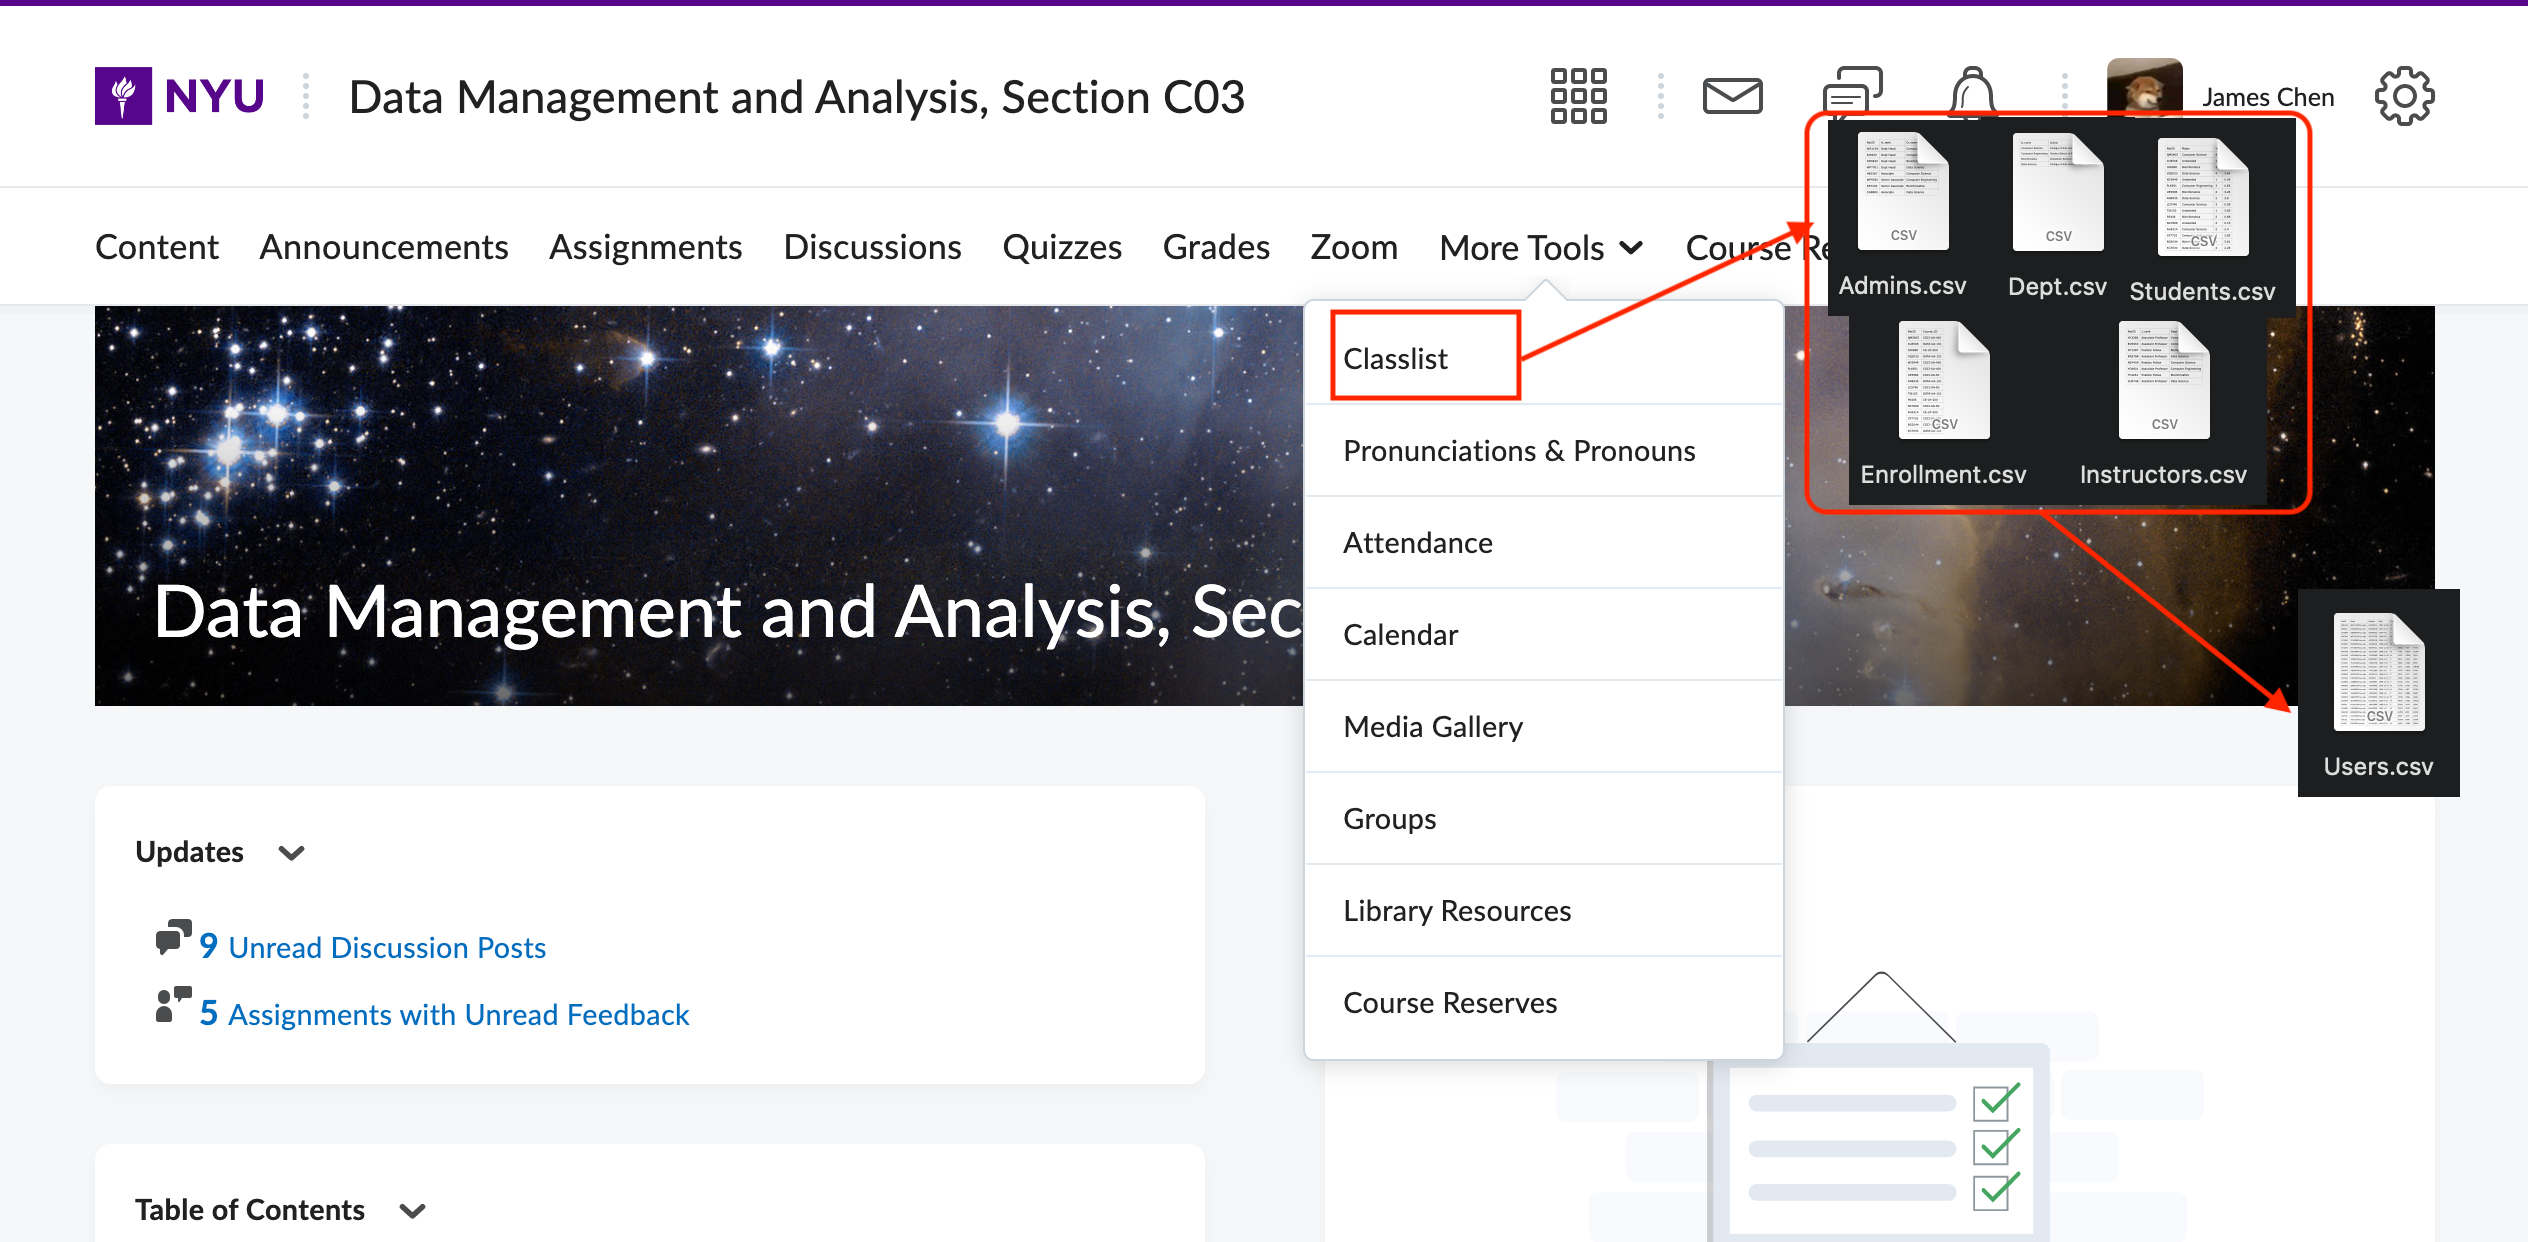
\includegraphics[width=\textwidth]{Intro3.png}
\end{figure}
\end{block}
\end{frame}

\section{Diagram}
\begin{frame}{Sections}
\begin{block}{Table of Content}
\begin{itemize}
    \item Introduction
    \item \textbf{Diagram}
    \item Data generation
    \item Query
\end{itemize}
\end{block}
\end{frame}

\begin{frame}{ER Diagram}
\begin{figure}[H]
    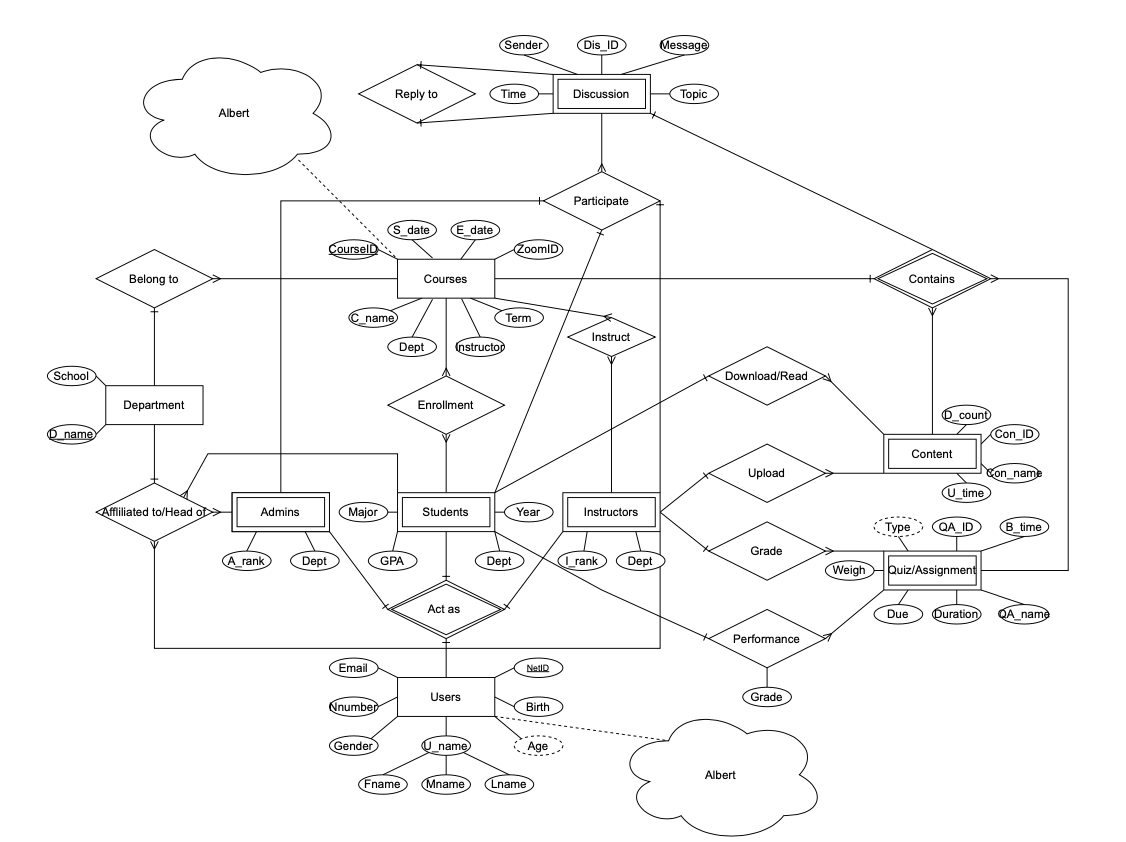
\includegraphics[width=\textwidth]{ER.png}
\end{figure}
\end{frame}

\begin{frame}{Table Diagram}
\begin{figure}[H]
    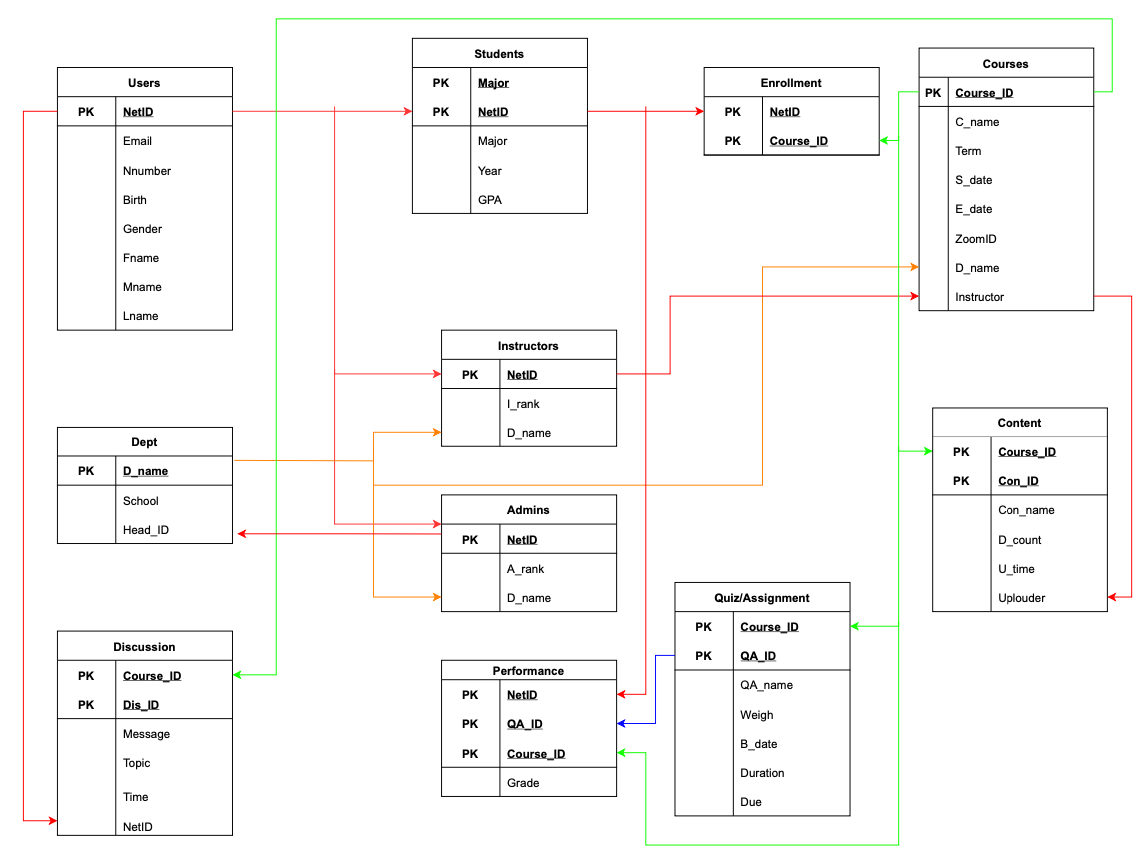
\includegraphics[width=\textwidth]{Table.png}
\end{figure}
\end{frame}

\section{Data}
\begin{frame}{Sections}
\begin{block}{Table of Content}
\begin{itemize}
    \item Introduction
    \item Diagram
    \item \textbf{Data}
    \item Query
\end{itemize}
\end{block}
\end{frame}

\begin{frame}{Data via Excel I}
\begin{block}{Random Data Generation -- Chars \& Nums}
\begin{figure}[H]
    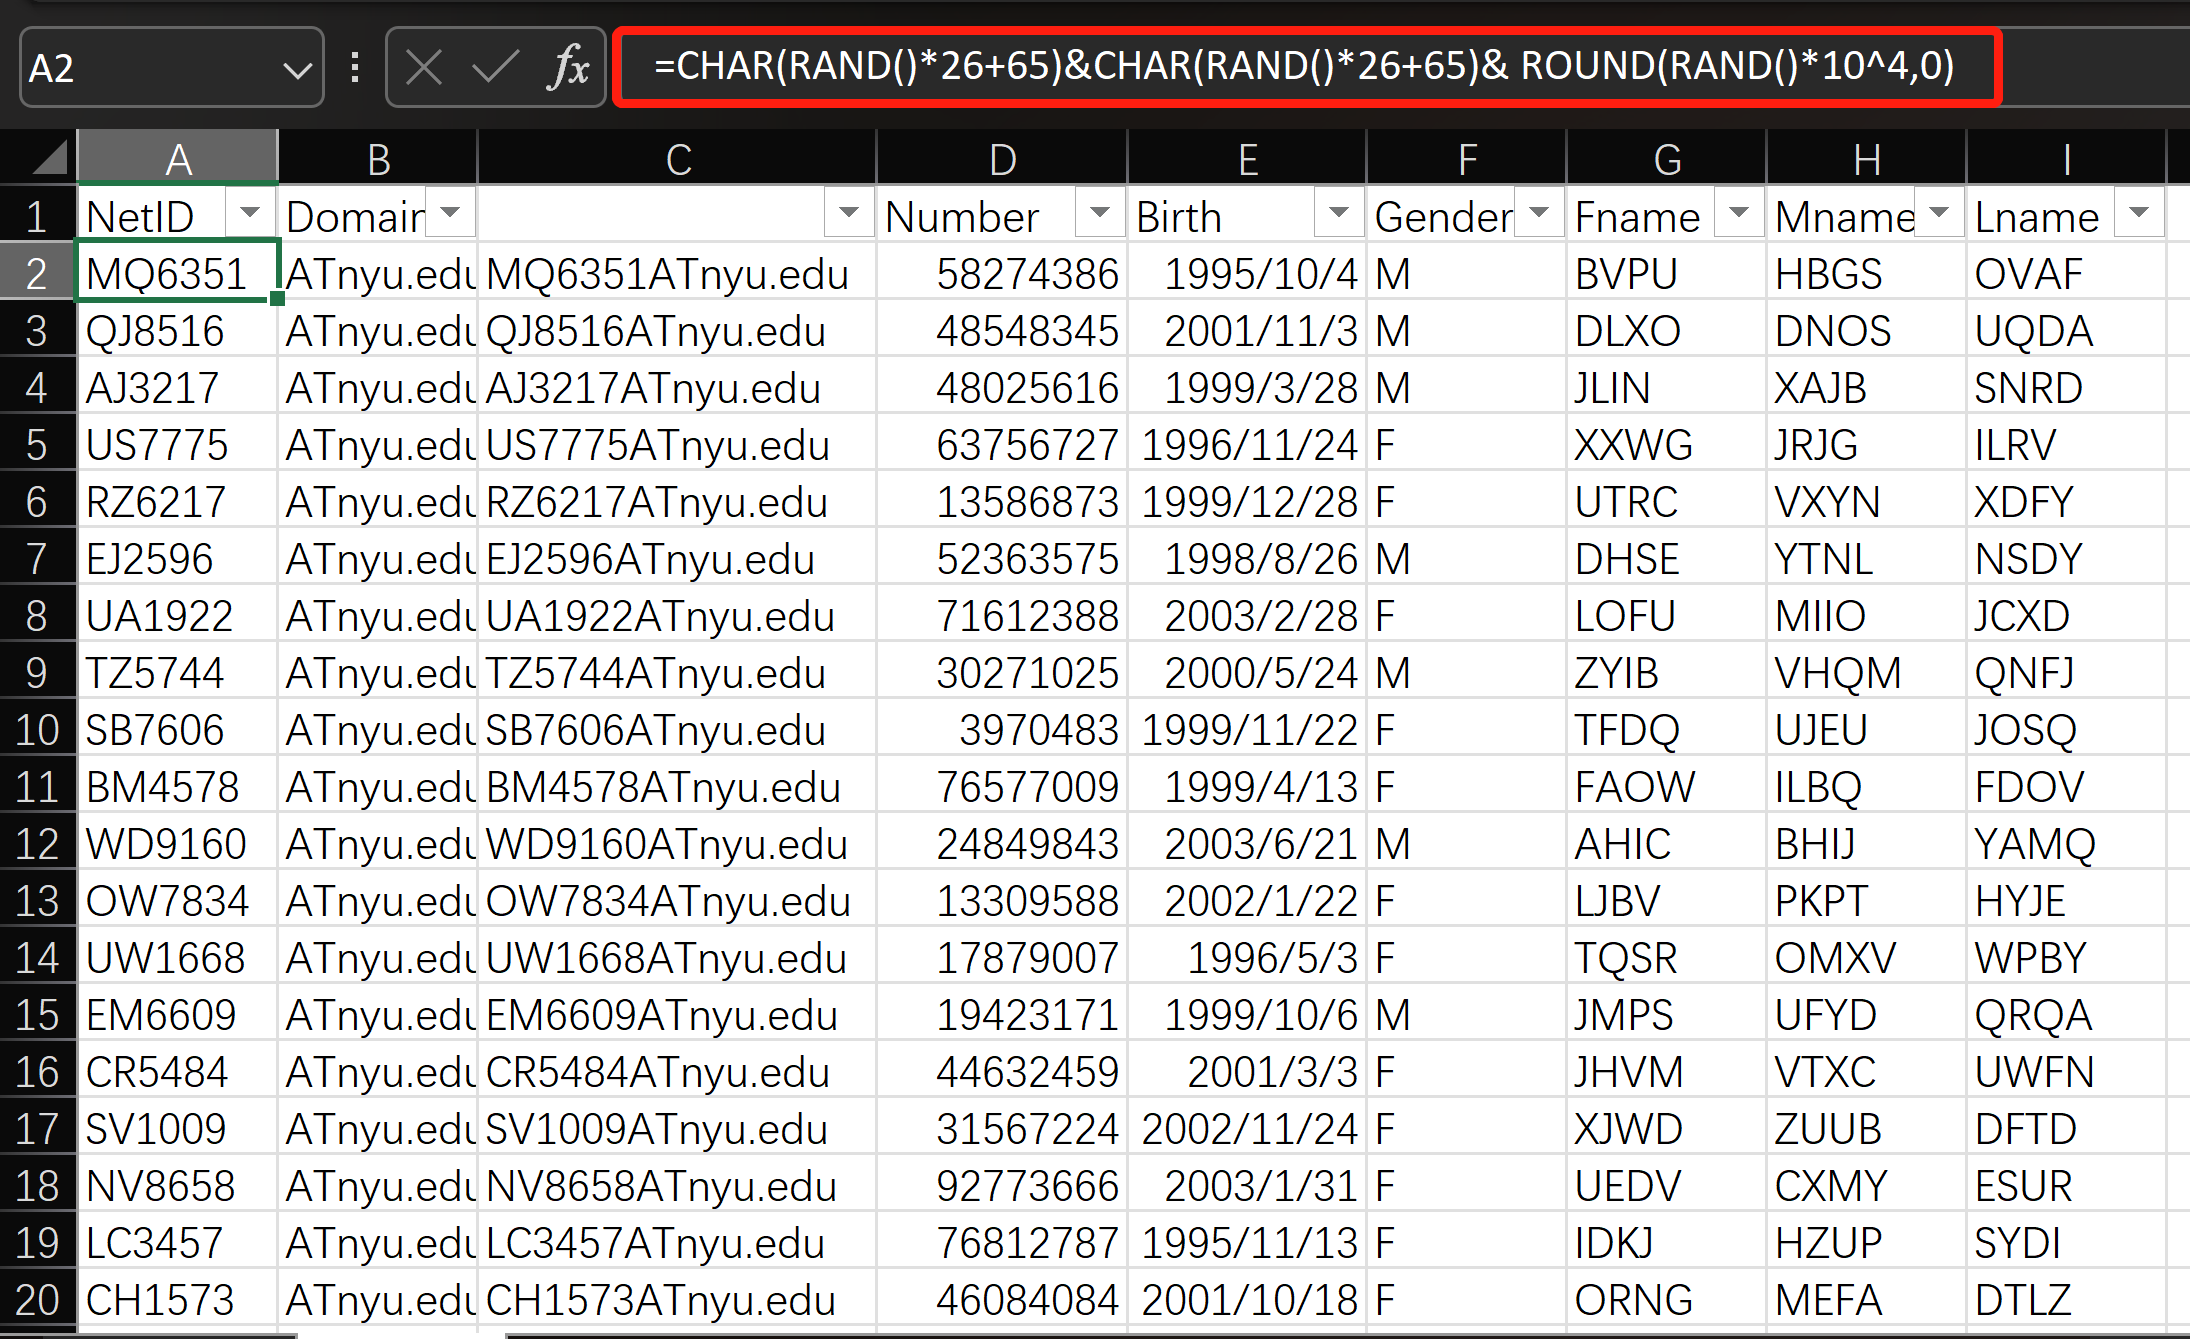
\includegraphics[width=\textwidth]{Data1.png}
\end{figure}
\end{block}
\end{frame}

\begin{frame}{Data via Excel II}
\begin{block}{Random Data Generation -- Dates}
\begin{figure}[H]
    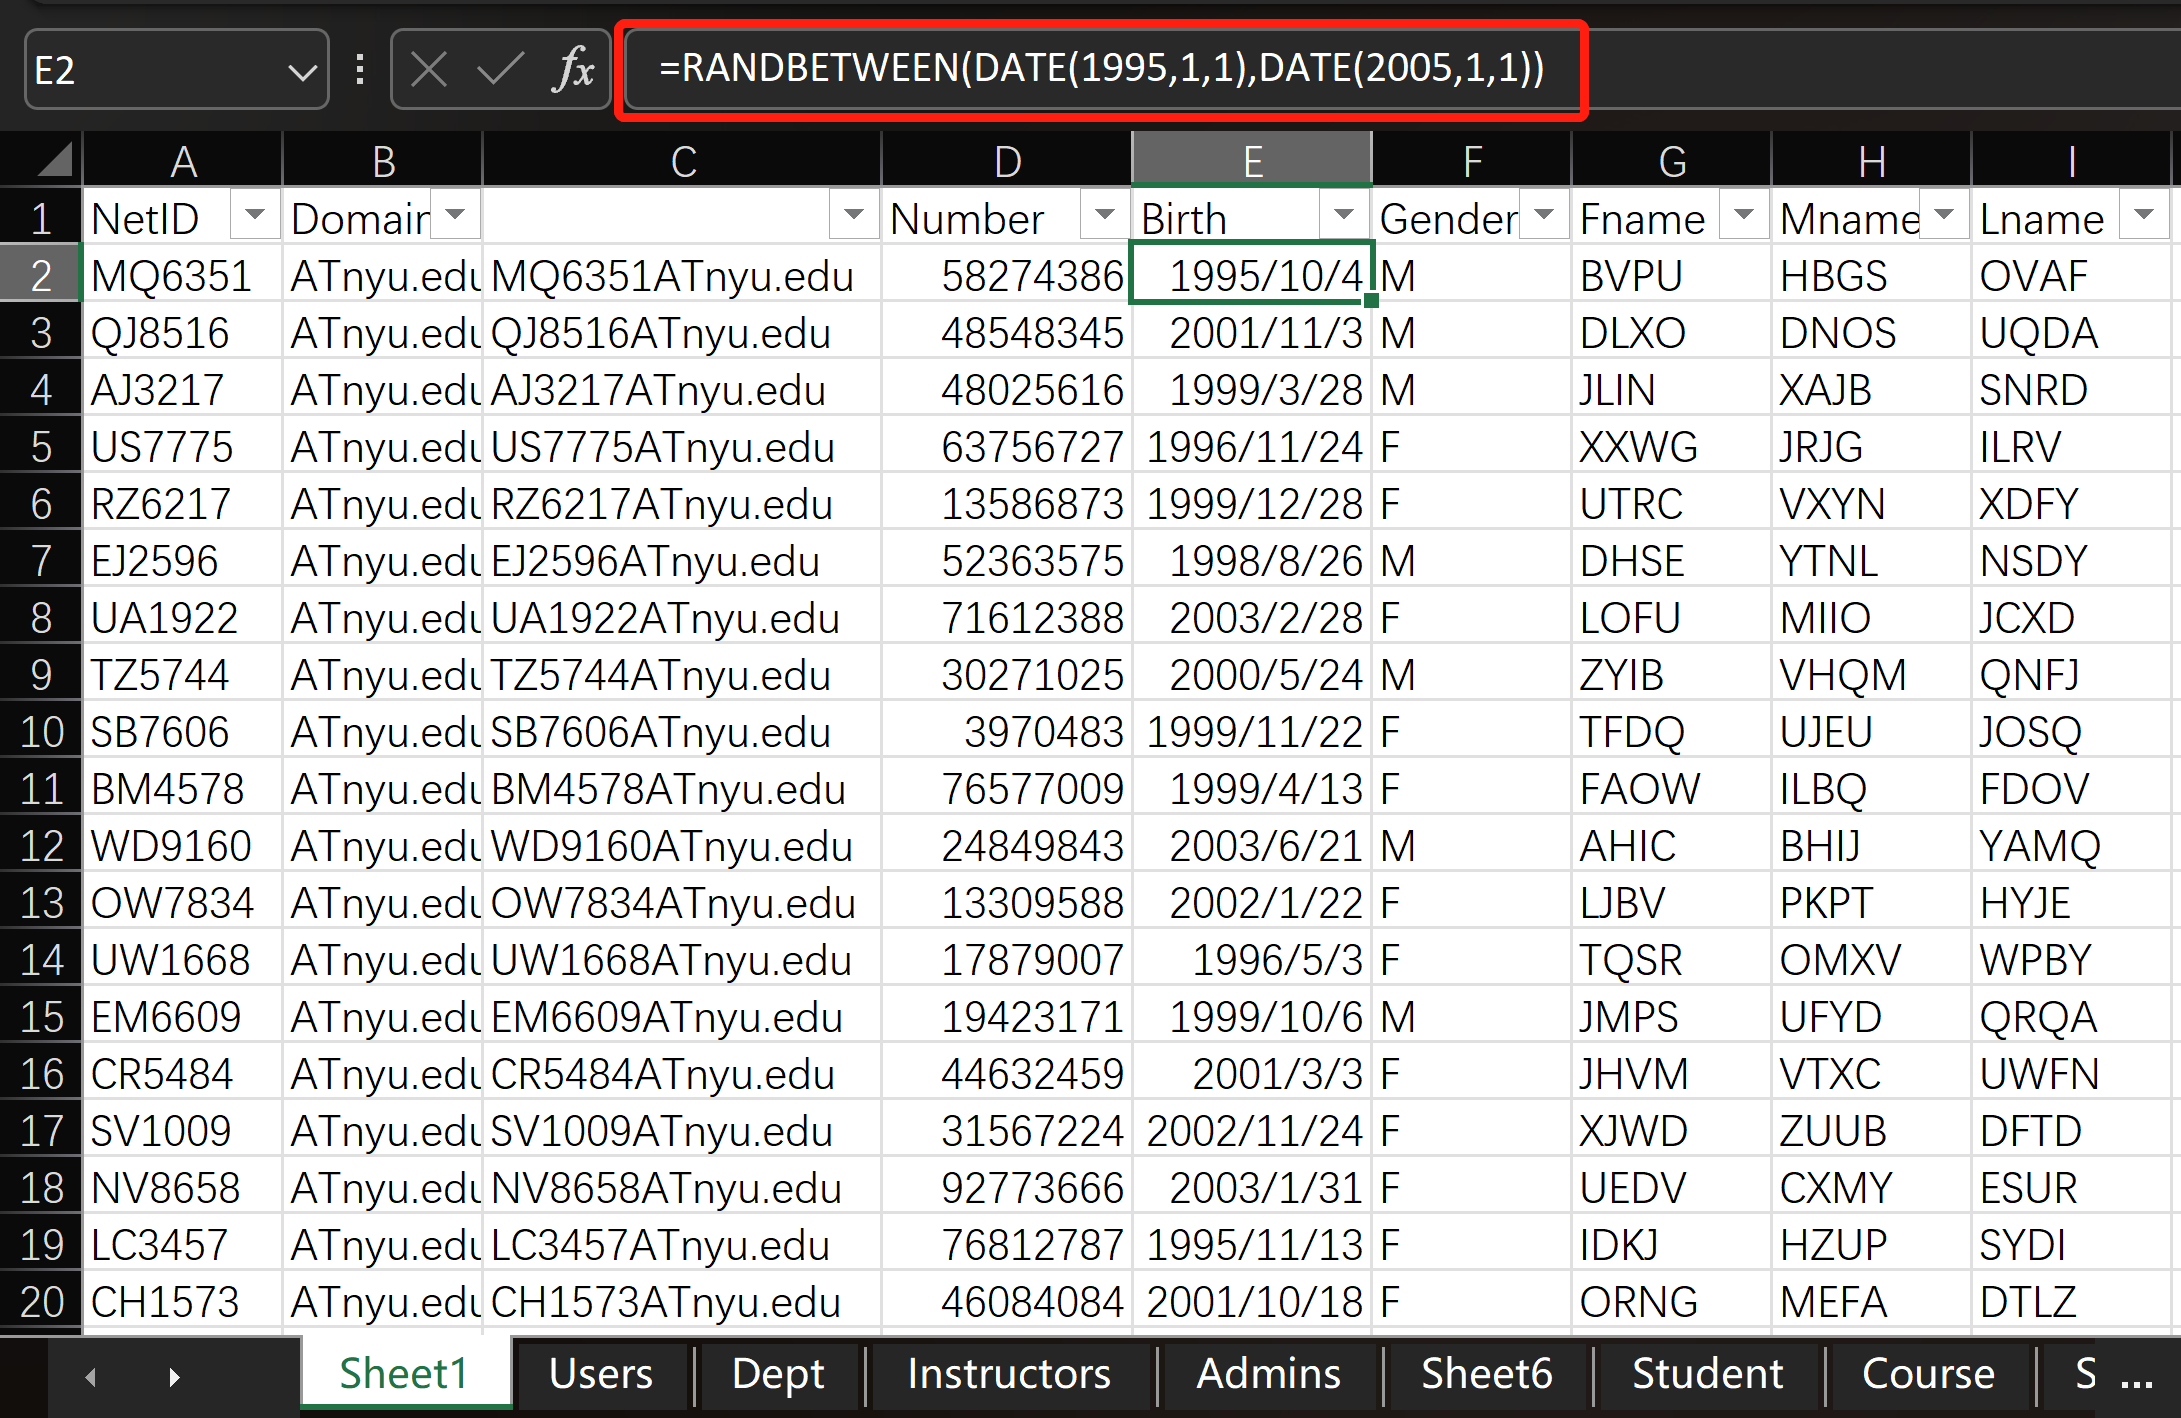
\includegraphics[width=\textwidth]{Data2.png}
\end{figure}
\end{block}
\end{frame}

\begin{frame}{Data via Excel III}
\begin{block}{Random Data Generation -- Normal Distribution}
\begin{figure}[H]
    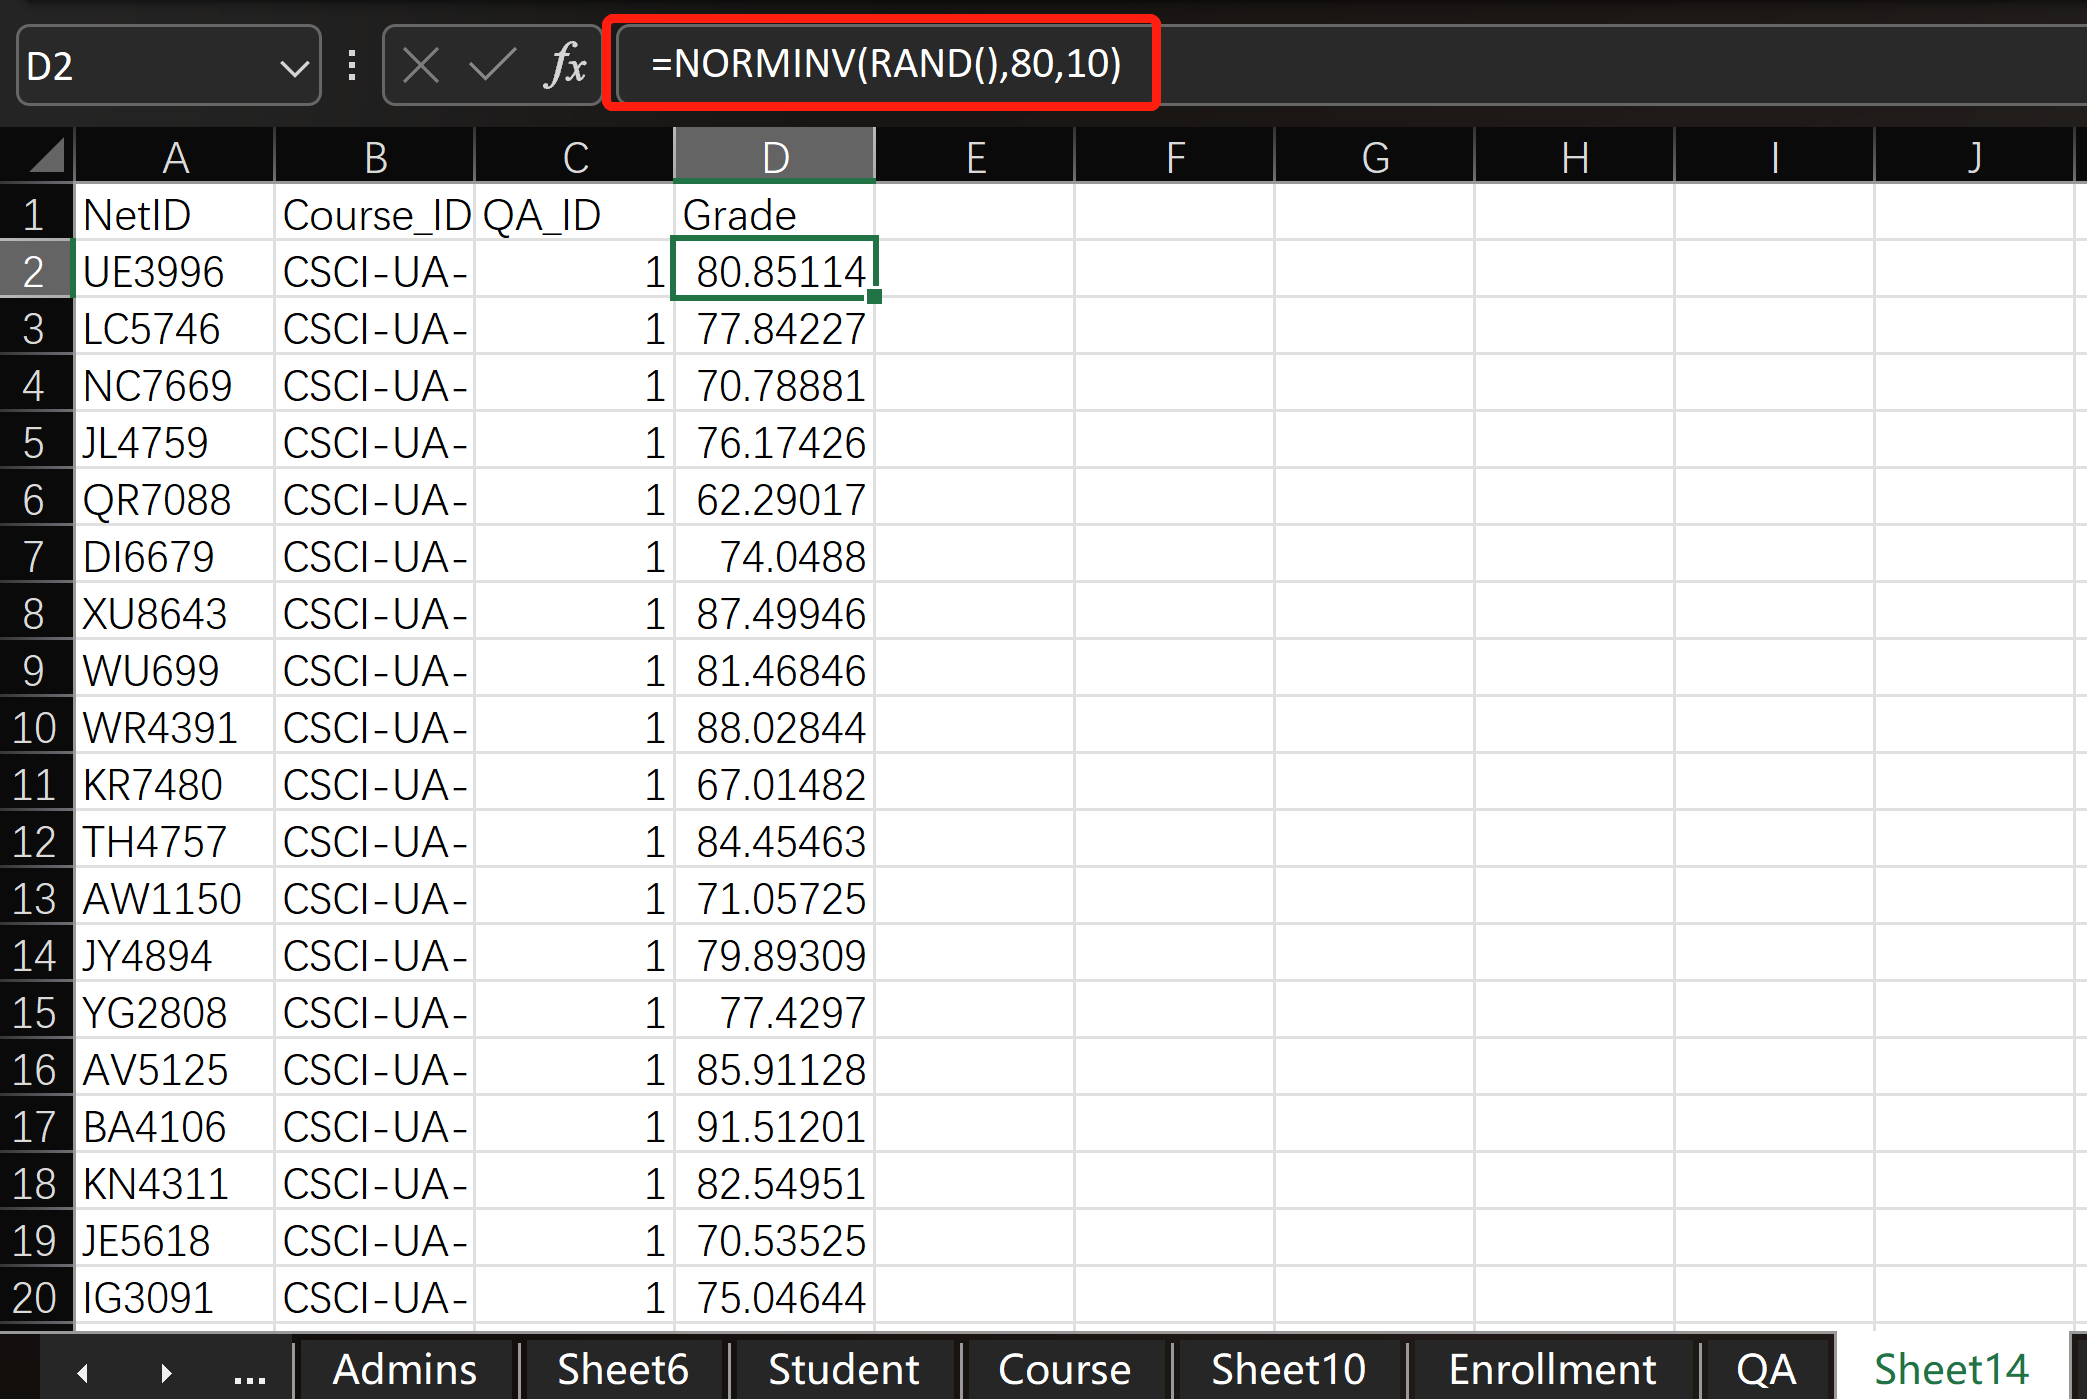
\includegraphics[width=\textwidth]{Data3.png}
\end{figure}
\end{block}
\end{frame}

\section{Query}
\begin{frame}{Sections}
\begin{block}{Table of Content}
\begin{itemize}
    \item Introduction
    \item Diagram
    \item Data
    \item \textbf{Query}
\end{itemize}
\end{block}
\end{frame}

\begin{frame}{Query I}
\begin{block}{Upper-class Students with Major Undecided}
    \inputminted[linenos]{mysql}{1.txt}
\end{block}
\begin{figure}[H]
    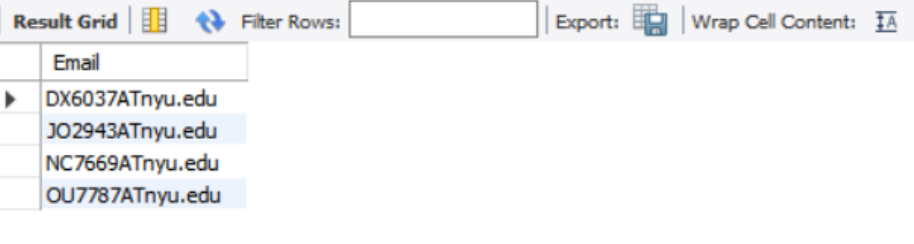
\includegraphics[width=\textwidth]{1.png}
\end{figure}
\end{frame}

\begin{frame}{Query II}
\begin{block}{Instructors with Courses in F22}
    \inputminted[linenos]{mysql}{2.txt}
\end{block}
\begin{figure}[H]
    
\includegraphics[width=\textwidth]{2.png}
\end{figure}
\end{frame}

\begin{frame}{Query III}
\begin{block}{Final Grade of CSCI-UA-60}
    \inputminted[linenos]{mysql}{3.txt}
\end{block}
\begin{figure}[H]
    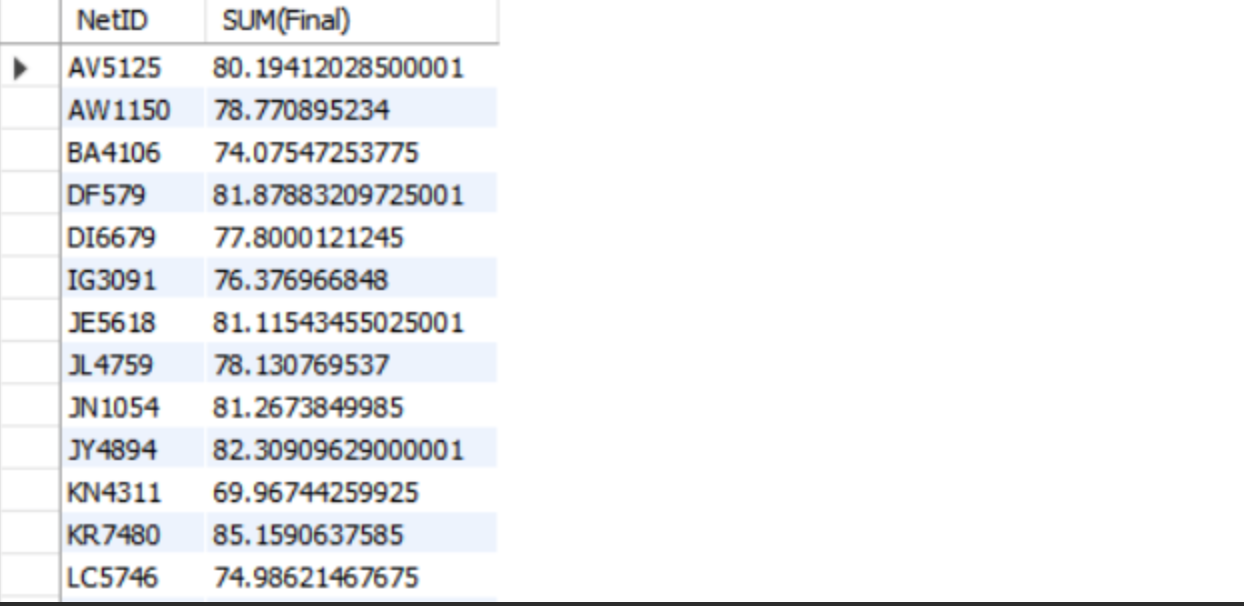
\includegraphics[width=\textwidth]{3.png}
\end{figure}
\end{frame}

\begin{frame}{Query IV}
\begin{block}{Discussion After the Release Time of HW2 of CSCI-UA-60}
    \inputminted[linenos]{mysql}{4.txt}
\end{block}
\begin{figure}[H]
    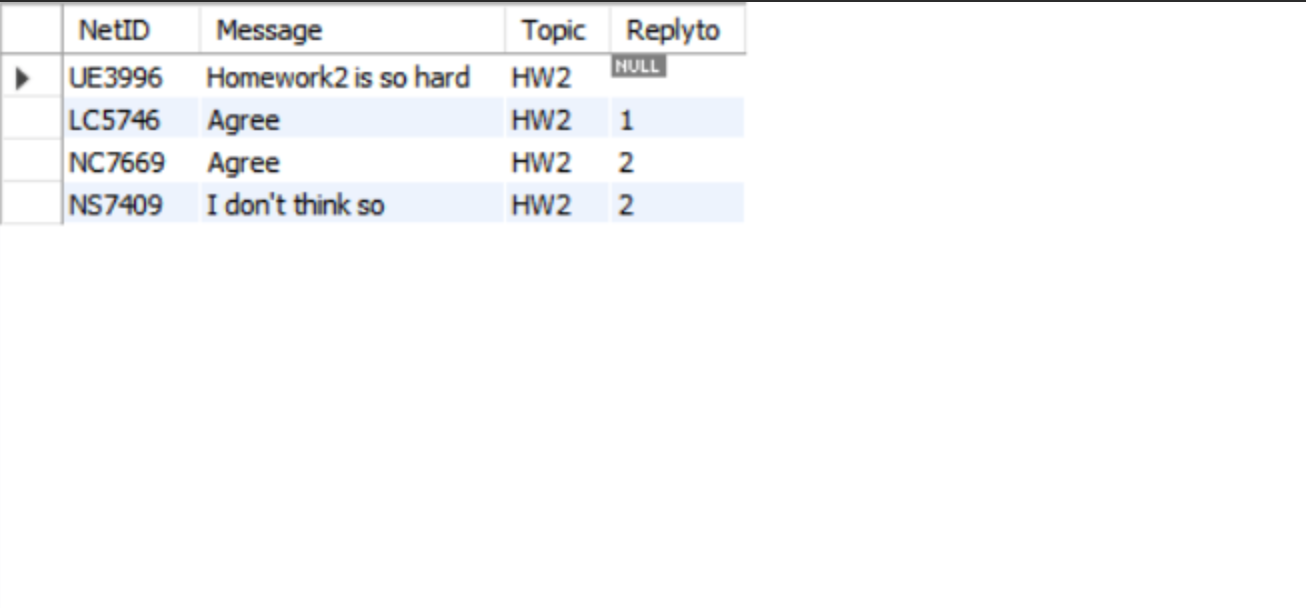
\includegraphics[width=\textwidth]{4.png}
\end{figure}
\end{frame}

\begin{frame}{Query V}
\begin{block}{Department Name, Head, and Faculty List}
    \inputminted[linenos]{mysql}{5.txt}
\end{block}
\begin{figure}[H]
    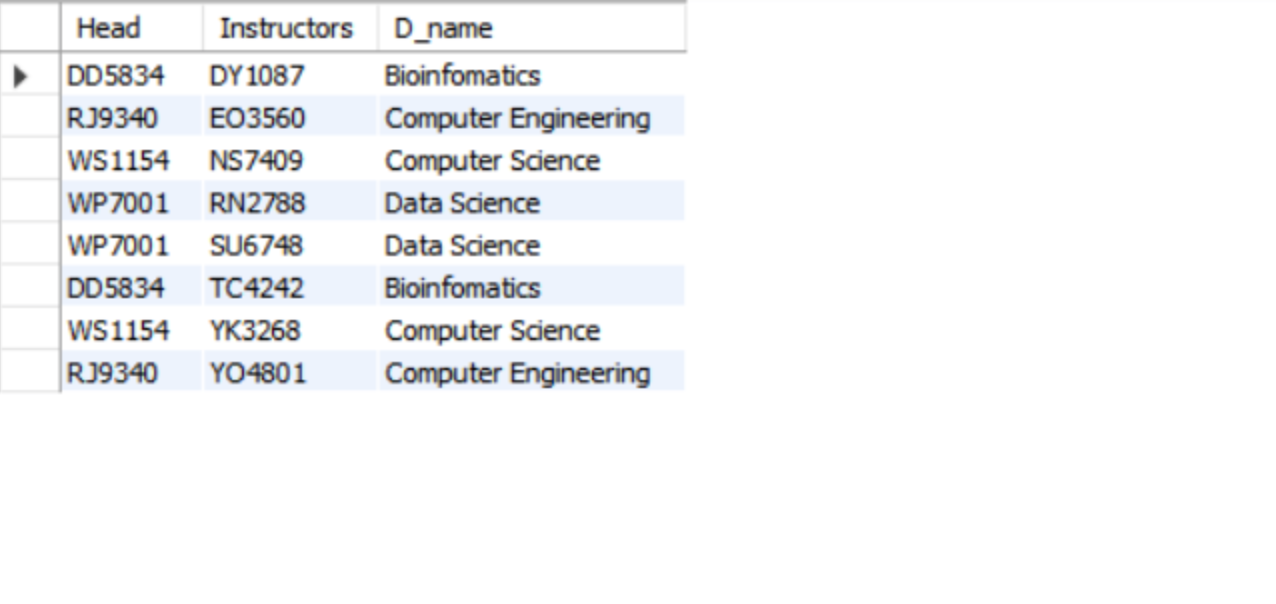
\includegraphics[width=\textwidth]{5.png}
\end{figure}
\end{frame}

\begin{frame}{Query VI}
\begin{block}{Most Popular Content}
    \inputminted[linenos]{mysql}{6.txt}
\end{block}
\begin{figure}[H]
    
\includegraphics[width=\textwidth]{6.png}
\end{figure}
\end{frame}


\section{Open Source}
\begin{frame}{Open Source}
\begin{block}{}
\begin{itemize}
    \item Code \& Data: https://github.com/zc2214/BrightspaceDB
    \item Diagram: https://drive.google.com/file/
    d/1UECFawvgM7R4tURZJR1Gbdee8NhyBABv/view?usp=sharing
    \item This \LaTeX \space Presentation Slides: https://www.overleaf.com/read/ntqmmdhhqjkq
\end{itemize}
\end{block}
\end{frame}

\section{Acknowledgments}
\begin{frame}{Acknowledgments}
\begin{block}{Acknowledgments}
We would like to express our sincere gratitude to our main instructor Dr. Anantha Padmanabha. Without your instruction, this project would not have been accomplished. Thanks Prof. Lihua Xu from NYU Shanghai for providing this very handy \LaTeX \space template.
\end{block}
\end{frame}

\end{document}